\section{Implementation} % (fold)
\label{sec:implementation}

Using the requirements set forth in Section~\ref{sec:dvpns} we can compile a list of contemporary technologies that can meet them and provide \acp{dvpn}. The protocols considered had to meet \ref{lst:num} criteria:
\begin{inparaenum}[\itshape 1\upshape)]
	\item can provide Ethernet \acp{ppvpn} between multiple sites, and
	\item protocol stack must be supported in hardware at time of writing.
	\label{lst:num}
\end{inparaenum}





what can provide what function for DVPNs?

\subsection{Contemporary Technologies} % (fold)
\label{sub:contemporary_technologies}

%\subsubsection{\acs{atm}} % (fold)
%\label{ssub:atm}
%For the sake of completeness, we will briefly look at \acs{atm}. \ac{atm} is a legacy protocol that has been used by operators to carry traffic over the internet backbone since the 1990s. Where as Ethernet and \ac{ip} are developed as packet-routing connection-less protocols, \ac{atm} is a cell-switched connection-oriented protocol. This poses a number of problems when trying to transport \ac{ip} over \ac{atm}. First, the variable length of the packets don't map efficiently to the fixed size cells of \ac{atm}. Drops of a single cell would cause the entire frame to become unusable. Then there is the added overhead of encapsulating \ac{ip} over \ac{atm}, which causes inefficient use of the network resources when compared to running an all \ac{ip} network. Finally, the \ac{qos} features of \ac{atm} are left unused \cite{atm}. These problems are some of the reasons that operators have moved away from \ac{atm} based backbones, to all \ac{ip} ones.
%
%% subsubsection atm (end)

\subsubsection{\acs{spb}} % (fold)
\label{ssub:spb}

\ac{spb} is an evolution of the original \acs{ieee} 802.1Q \ac{vlan} standard. \ac{vlan} tags have been in use in the networking world for a long time and provide decent separation in campus networks. However, when \ac{vlan}-tagging was done at the customer network, the carrier couldn't separate the traffic from different customers anymore. This resulted in 802.1Qad or Q-in-Q which added an S-\ac{vlan} tag to separate the client \acp{vlan} from the \ac{sp} \acp{vlan} in the backbone. This was usable for the Metro Ethernet networks for awhile but when \acp{sp} started providing this services to more and more customers, their backbone switches could not keep up with the clients \ac{mac} addresses.

To provide the required \acs{mac} scalability problem \ac{pbb} (802.1Qay or \ac{mac}-in-\ac{mac}) was introduced. It encapsulates the whole Ethernet frame on the edge of the carrier network and forwards the frame based on the Backbone-\ac{mac}, Backbone-\ac{vlan} and the I-SID. The I-SID is a Service Instance Identifier, which with 24 bits is able to supply the carrier with 16 million separate networks. The downside of \ac{pbb} remained one that is common to all Layer 2 forwarding protocols: the possibility of loops. Preventing them requires \ac{stp} which will disable links to get a loop-free network. Disadvantages of \ac{stp} include the relatively long convergence time and inefficient use of resources due to the disabled links. This final problem was solved by using \acs{isis} as a routing protocol to distributed the topology and creating \acp{spt} originating from each edge device. This is called \ac{spb} or 802.1aq.

\ac{spb} benefits from the maturity of the Ethernet protocol by reusing protocols for \ac{oam} and \ac{pm}. This allows for fast error detection and extensive troubleshooting tools by using the \ac{ieee} 802.1ag and \ac{itut} Y.1731 standards respectively. The \ac{isis} implementation has also been adapted to rapidly detect errors however, no fast recovery function has been defined, besides complete \ac{isis} reconvergence. This would result in a traffic impact of several hundreds of milliseconds in large networks \cite{spb-nanog}. 

However, due to its Ethernet \acs{stp} forwarding-based nature it lacks \ac{te} features. The paths that the \ac{vpn} traffic takes are not explicitly configureable and provide limited scalability due to limited amounts of available paths (or trees in this case). This also negatively affects its \ac{ecmp} functionalities, which are limited by the available paths as well. However, using extensible \ac{ect} algorithms, future, additional algorithms with multiple paths maybe introduced \cite{rfc6329}.

Provided that \ac{isis} has been configured on all provider devices, Figure~\ref{fig:spb-stack} illustrates the interfaces needed to provision a \ac{dvpn} in \ac{spb}. First, the I-SID has to be defined on all \acp{pe}, which in turn will setup \acp{spt} towards the other participating \acp{pe}. The member \ac{ce} ports then need to be added to the I-SID after which the \acp{vpn} is established. The rate limiting of the \ac{ce} ports is a vendor-specific feature, however and may vary per hardware platform.

\begin{figure}[!h]
	\centering
	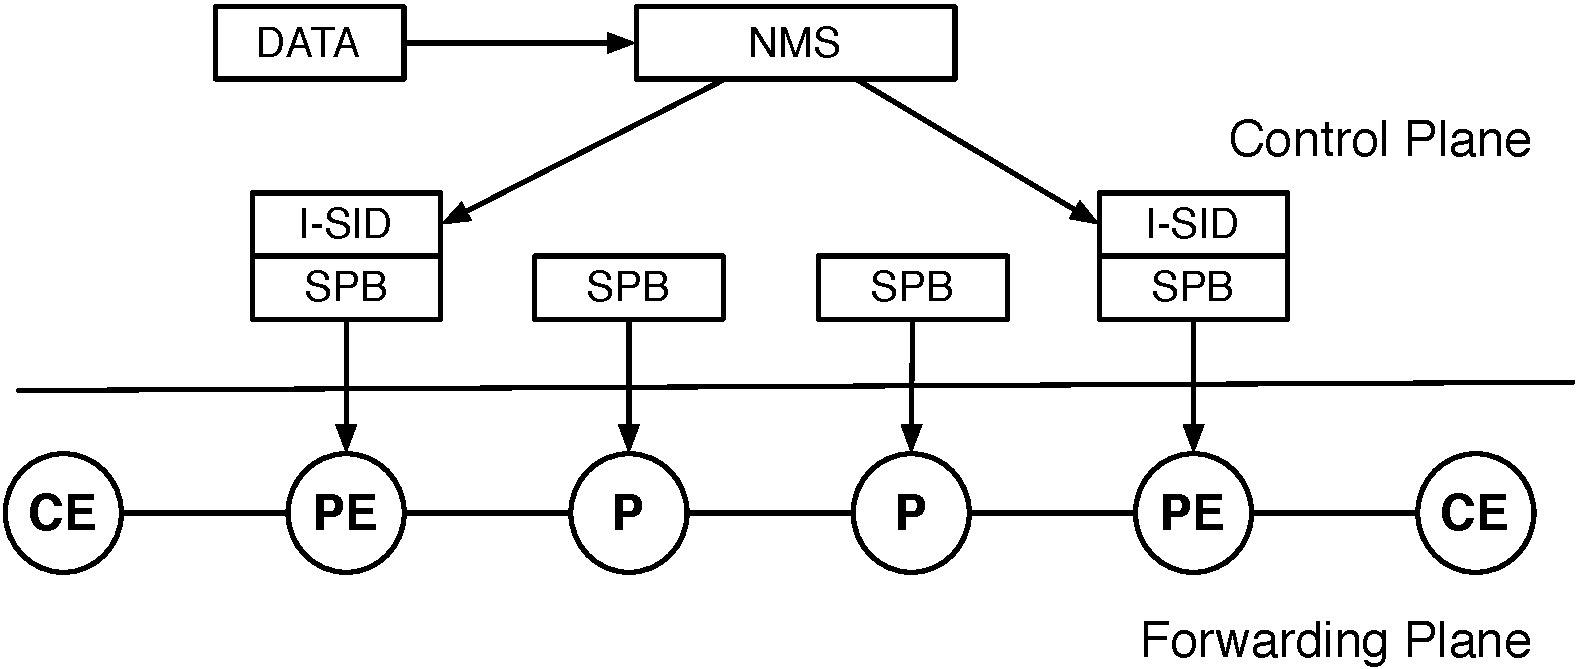
\includegraphics[width=9cm]{./includes/spb-stack.pdf}
	\caption{Provisioning a \ac{dvpn} using \ac{spb}.}
	\label{fig:spb-stack}
\end{figure}


% subsubsection spb (end)

\subsubsection{\acs{mpls}} % (fold)
\label{ssub:mpls}

\ac{mpls} is known for its scalability and extensibility. Over the past decade additions have been made to the original specification to overcome a plethora of issues within carrier networks. This initially started with trying to implement fast forwarding in legacy switches using labels (or tags) at the start of the frame \cite{tag-switching}. When this issue became surmountable using new hardware, \ac{mpls} had already proven to be capable of transporting a wide arrange of protocols on the carrier backbone network, all the while also providing scalability, \ac{te} and \ac{qos} features to the operators.

\ac{mpls} itself is more a way of forwarding frames through the network, without facilitating any topology discovery, route determination, resource management, etc. These functions are left to a stack of other protocols. Without \ac{ip} reachability throughout the network these protocols cannot exchange traffic and so, as a prerequisite, \ac{mpls} relies on an \ac{igp} like \ac{ospf} to discovery the topology.

The distribution of labels has to be facilitated as well, which is done using \ac{ldp} and/or \ac{rsvp}. These protocols run between each device in the path between two \acp{pe} and exchange the labels that the will assign to a certain path, thereby setting up a \ac{lsp}. \ac{ldp} does this by distributing its labels from the egress \ac{pe} up towards the ingress \ac{pe} based on \ac{igp} costs. \ac{rsvp}, on the other hand, signals its paths from the ingress \ac{pe} towards the downstream \ac{pe} based on constraints, potential explicit hops or as a last resort using the \ac{igp} next hop. Label distribution is still determined from egress to ingress, but the actual path is determined at the head-end. To determine the best path to take, \ac{rsvp} uses the \ac{cspf} algorithm which can take into account link characteristics like bandwidth or \ac{frr} support. This allows \ac{rsvp} \acp{lsp} to take more well informed paths through the network and together with support for defining explicit paths, allows for granular \ac{te} features which \ac{ldp} lacks. Both \ac{ldp} and \ac{rsvp} also allow for the use of multiple paths over the network to share traffic load towards a \ac{pe}.

The aforementioned \ac{frr} feature is unique to \ac{rsvp} and provides the network with fast failure recovery. It does so by preprovisioning a so-called backup \ac{lsp} next to the primary \ac{lsp}. When a failure is detected on the primary \ac{lsp}, traffic is immediately shifted towards the standby path, yielding a sub-50ms failover. Obviously, this value also depends on the time it takes for the failure to be detected. Therefore it is important to have some sort of detection mechanism in place. One that is commonly used and integrates with \ac{ospf} is \ac{bfd}. This protocol sets up sessions between devices and triggers an alarm when the session does not behave as expected. At which point \ac{frr} kicks in.

\acp{vpn} are also provided by additional protocols. Layer 3 \acp{vpn} make use of \ac{bgp} to distribute client prefixes to the edges of the carrier network. The core is only concerned with the forwarding of labels and has now knowledge of these \acs{ip} prefixes. Layer 2 \acp{vpn} make use of \ac{vpls}, a service which encapsulates the entire Ethernet frame and pushes a label to it to map it to a certain separated network. Again, the core is only concerned with the labels and only the edges need to know the clients \acs{mac} addresses. When setting up a \ac{vpls} instance (a \acp{vpn}), \ac{ldp} sessions are setup between all \acp{pe} part of the same \ac{vpls} instance. Consecutively, the \acp{pe} will exchange their chosen labels for that instance between each other.

The \acp{cmac} in a \ac{vpls} instance are normally learned through the data plane. That is, when a frame comes in from a \ac{ce}, the \ac{pe} learns the \ac{sa} behind the corresponding port. If it doesn't know the \ac{da}, it will flood the frame to other \acp{pe} with member ports in that instance. These \acp{pe} in turn learn the \ac{sa} as well behind the ingress \ac{pe}. When a large number of \acp{cmac} are present within a \ac{vpls} instance this can cause a lot of broadcast traffic, specifically \ac{arp} traffic. To solve this, the \ac{evpn} standard has been proposed \cite{evpn}. This technique provides \ac{mac} learning in the control plane by exchanging learned \acp{cmac} between \acp{pe} using Multi-Protocol \ac{bgp}. Additionally it may also learn the \ac{ip} address associated with the \ac{cmac} and distribute that as well. Thereby being able to act as an \ac{arp} proxy, as earlier illustrated in Figure~\ref{fig:arp-proxy}.

The different protocols all depend on each other, as illustrated in Figure~\ref{fig:mpls-stack}. Each \ac{pe} device runs this stack, while \ac{p} devices run a subset which is shaded. 

\begin{figure}[!h]
	\centering
	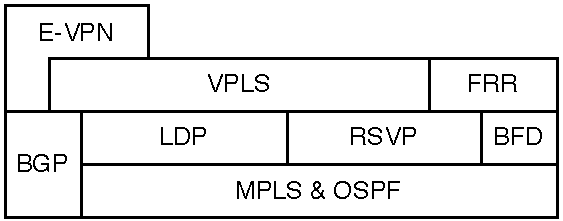
\includegraphics[width=7cm]{./includes/mpls-stack.pdf}
	\caption{Dependency stack of \ac{mpls}-related technologies.}
	\label{fig:mpls-stack}
\end{figure} 

To configure a \ac{dvpn} using \ac{mpls} first the participating \acp{pe} need to be configured with the new \ac{vpls} instance to which the member \ac{ce} ports will be added. Next, constraints are defined by the \ac{nms}, which can be in the form of an explicit route to make a static route or by defining loose constraints based on bandwidth limits which can be used the \ac{cspf} algorithm. Using these constraints, paths are installed at each \ac{pe} towards every other participating \ac{pe}. These paths are then added to the \ac{vpls} instance, allowing \ac{ldp} sessions to be setup between the \acp{pe}. Next, for \ac{frr}, backup \acp{lsp} need to defined similarly to the primary \ac{lsp} but over a different path, which can again be done using constraints to exclude the other links. Utilization of the links in the network has to be monitored as well and when a path has a link which is nearing capacity, new \acp{lsp} have to be provisioned and some \ac{vpls} paths move to those \acp{lsp}. And finally the ingress traffic on the \ac{ce} ports need to be rate limited. This procedure again, is not standardized and is dependent on support of the hardware.

The procedure above implies that the backbone network has been setup with the following protocols and features already enabled: \ac{ip} addressing, \ac{ospf} routing, \ac{mpls} forwarding, \ac{rsvp} with \ac{frr} and \ac{bfd}. After initial setup of the backbone network the \ac{nms} is only concerned with the \acp{pe}, as can also be seen in Figure~\ref{fig:nms-stack}.

\begin{figure}[!h]
	\centering
	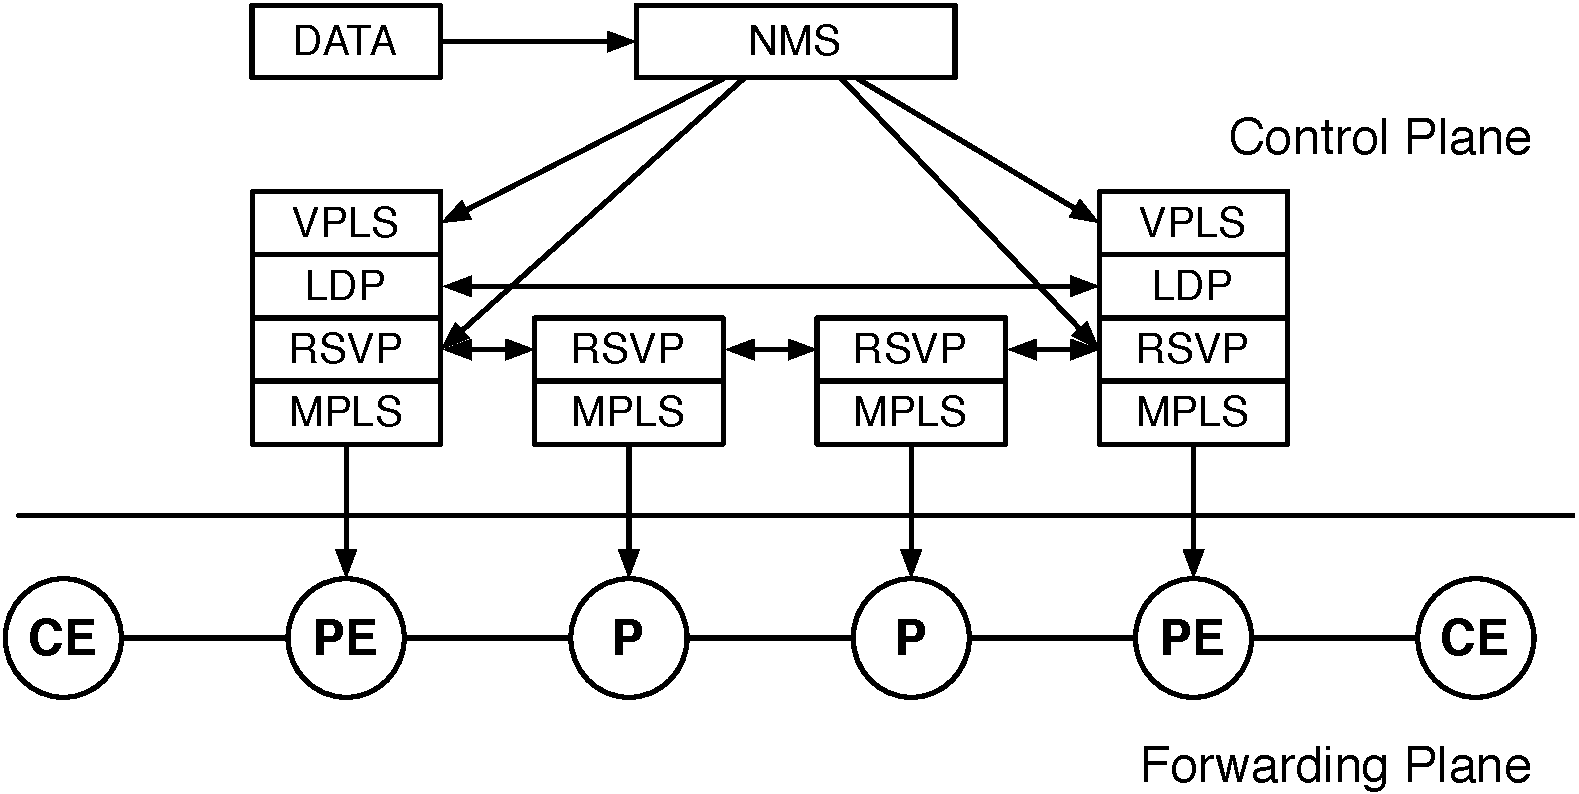
\includegraphics[width=9cm]{./includes/nms-stack.pdf}
	\caption{Provisioning a \ac{dvpn} using \ac{mpls}.}
	\label{fig:nms-stack}
\end{figure}

% subsubsection mpls (end)

% subsection contemporary_technologies (end)

\subsection{OpenFlow} % (fold)
\label{sub:openflow}

Section~\ref{sec:introduction} gave a short introduction into what \ac{sdn} and OpenFlow entail and what it promises in terms of cost savings and agility. \acl{sdn} is the general principle of designing flexible networks using open interfaces towards the hardware. The complete architecture is being generalized by the networking industry within the OpenDaylight project \cite{opendaylight}. Looking at OpenFlow itself from a more technical point of view, it boils down to a protocol used to program the forwarding plane in networking devices from a centralized server called the `controller'. 

The momentum that \ac{sdn} is getting might be explained by a general need for change in the networking industry. Operators primarily want to get more control over their networks, something which using the current stack of protocols is relatively complicated to get. The original \acs{osi} reference model \cite{zimmermann} touches on the ``Management Aspects'' of each layer in the model, a way for management entities in the highest layer to control the behavior of lower layers. Unfortunately in the swift evolution of \ac{tcp}/\ac{ip}, these management interfaces are often limited or absent all together. 

This means that through protocols such as \ac{rsvp}-TE, operators are trying to get control over the lower levels of the networking stack. 

The OpenFlow controller provides operators with an alternative to these interfaces, namely a programmable forwarding plane. 

\begin{table}[h]
	\centering
	\begin{tabular}{r|cccc}
	 			& 1.0 & 1.1 & 1.2 & 1.3\\
	\hline
	VLAN Tags 	& x & x & x & x \\
	Q-in-Q Tags &   & x & x & x \\
	MPLS Tags 	&   & x & x & x \\
	PBB Tags 	&   &   &   & x \\
	Groups 		&   & x & x & x \\
	Metering 	&   &   &   & x \\
	\end{tabular}
	\caption{Comparison of OpenFlow version regarding key features for \acp{dvpn}.}
	\label{tb:of-versions}	
\end{table}

The OpenFlow specification has been through a few revisions since it was first proposed. In the first version tagging of traffic was only support using a single \acs{vlan} tag. Version 1.1 added matches for \ac{mpls} and Q-in-Q tags, and version 1.3 could also match \ac{pbb} tags. Also not included in version 1.0 were mechanisms to allow for fast failover and \ac{ecmp}. These were added in version 1.1 by introducing logical groups of ports to which a flow entry can forward the frame. However, to support fast failover a \textsl{liveness monitoring} technique will need to be implemented supported by the switch. This could simply be the physical link state or more intricate tools, e.g.\ \ac{bfd}. See also Table~\ref{tb:of-versions}. 

\begin{figure}[!h]
	\centering
	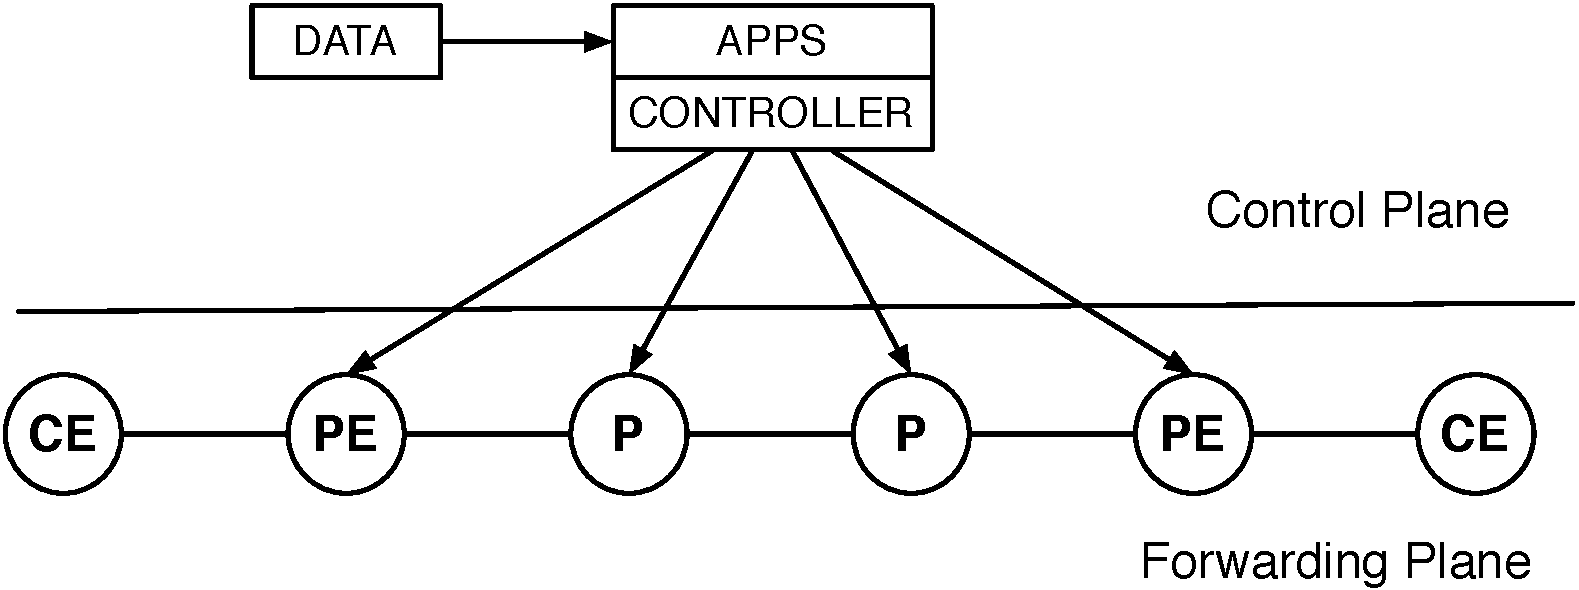
\includegraphics[width=9cm]{./includes/nms-stack-of.pdf}
	\caption{Provisioning a \ac{dvpn} using OpenFlow.}
	\label{fig:nms-stack-of}
\end{figure}

% subsection openflow (end)

The features and limitations of the three discussed technologies are given in Table~\ref{tb:reqs}. They are compared to the list of requirements as discussed in Section~\ref{sec:dvpns}. Section~\ref{sec:results} will continue with an evaluation of the three architectures.

\begin{table}[h]
	\centering
	\begin{tabular}{r|lll}
	 & \acs{spb} & \acs{mpls} & OpenFlow / \acs{sdn}\\
	\hline
	Tagging of VPN Traffic & \acs{pbb} & \acs{vpls} & \acs{pbb} / \acs{mpls}\\
	MAC Scalability & yes & yes & yes\\
	Topology Discovery & \acs{isis} & \acs{ospf} & application\\
	Path Provisioning & \acs{spt} & \acs{rsvp} / \acs{ldp} & application\\
	Traffic Engineering & no & \acs{rsvp} & application\\
	\ac{ecmp} & limited & yes & yes, using Groups\\
	\ac{bum} limiting & dependent on \acs{hw} & dependent on \acs{hw} & yes, using Metering\\
	Exchange \acsp{cmac} & no & \ac{evpn} (draft) & application\\
	Traffic Rate Limiting & dependent on \acs{hw} & dependent on \acs{hw} & yes, using Metering\\
	Fast Failover & no & \acs{frr} & yes, using Groups\\
	\acs{oam} & 802.1ag & \acs{lsp} Ping / \acs{bfd} & application\\
	\hline
	Forwarding Decision & \acs{pbb} tags & \acs{mpls} labels & flow entry \\
	\ac{bum} traffic handling & flood & flood & sent to controller\\
	\end{tabular}
	\caption{Required features and corresponding available technologies.}
	\label{tb:reqs}
\end{table}

% section implementation (end)
